
\documentclass[spanish]{article}
\usepackage[a4paper]{geometry}  % for page size and margin settings
\geometry{left=3.5cm, right=1cm, top=3cm, bottom=1.5cm}
\usepackage{graphicx}		    % for insert images
\usepackage[es-tabla]{babel} 	% for spanish titles
\usepackage{mathtools}          % for greek math symbol formatting
\usepackage{enumitem}           % for control of 'enumerate' numbering
\usepackage{listings}           % for control of 'itemize' spacing
\usepackage{indentfirst}		% package to make first paragraph always indented
\usepackage{hyperref}           % page numbers and '\ref's become clickable
\usepackage{bm}					% for bold maths
\usepackage{setspace}			% for setting interline spacing
\usepackage{amsmath}			% for matrices
\usepackage{tikz} 				% for graphs
\usepackage{multirow}			% for tables
\usepackage{float}				% to manually select placement of tables
\usepackage{autobreak}          % to automatically fit equations to page width
\usepackage{soul}				% for highlighting


\usetikzlibrary{babel}		    % for draw arrows in tikz using babel spanish
\doublespacing					% for use double interline spacing
\bibliographystyle{ieeetr}
\numberwithin{figure}{subsection}
\numberwithin{equation}{subsection}
\numberwithin{table}{subsection}

% TITLE VARIABLES 

\def\thesistitle{Incorporación de covariables que varían en el tiempo a un modelo mixto}
\def\thesisauthorfirst{\textbf{Esteban Cometto}}
\def\thesissupervisorfirst{Noelia Castellana}
\def\thesissupervisorsecond{Cecilia Rapelli}
\def\thesisdate{\today}

%% OTHER USEFUL VARIABLES 

\def\npatients{560}

%% FOR PDF METADATA
\title{\thesistitle}
\author{\thesisauthorfirst\space\thesisauthorsecond}
\date{\thesisdate}

\begin{document}

\begin{titlepage}
    \newcommand{\HRule}{\rule{\linewidth}{0.5mm}}
	\center
	\textsc{\Large Universidad Nacional de Rosario}\\[.7cm]
	
\includegraphics[width=25mm]{img/fceye-unr.png}\\[.5cm]
	\textsc{Facultad de Ciencias Económicas y Estadística}\\[0.5cm]
	\textsc{Tesina}
	
	\HRule \\[0.4cm]
	{ \huge \bfseries \thesistitle}\\[0.1cm]
	\HRule \\[.5cm]
	
	\begin{minipage}{0.6\textwidth}
	\large
	\textit{Autor:}	\thesisauthorfirst
	\end{minipage}
	\\[.6cm]
	\begin{minipage}{0.6\textwidth}
	\textit{Directora:} 	\thesissupervisorfirst \\[.2cm]
	\textit{Codirectora:} 	\thesissupervisorsecond
	\end{minipage}
	\\[4cm]
	\vfill
	{\large \thesisdate}\\
	\clearpage
\end{titlepage}

\newpage
\tableofcontents

\newpage
\section{Introducción}

Los datos longitudinales están conformados por mediciones repetidas sobre una
unidad, las cuales pueden surgir por ser medidas en diferentes momentos o
condiciones. Su principal objetivo es estudiar los cambios en el tiempo y los
factores que influencian el cambio. 

Los modelos mixtos permiten ajustar datos con estas características, donde la
respuesta se modela por una parte sistemática que está compuesta por una
combinación de características poblacionales que son compartidas por todas las
unidades (efectos fijos), y una parte aleatoria que está constituida por efectos
específicos de cada unidad (efectos aleatorios) y por el error aleatorio, las
cuales reflejan las múltiples fuentes de heterogeneidad y correlación entre y
dentro de las unidades.

En estos modelos pueden incorporarse covariables. Las mismas se pueden
clasificar en 2 categorías: covariables no variables en el tiempo (CNVT) y
covariables variables en el tiempo (CVT). La naturaleza diferente de estas
covariables conduce a considerar distintos enfoques para cada una de ellas en el
análisis.

Las CNVT son variables independientes que no tienen variación intra-unidad, es
decir, que el valor de la covariable no cambia para una unidad determinada en
el estudio longitudinal. Este tipo de covariables se pueden utilizar para
realizar comparaciones entre poblaciones y describir diferentes tendencias en el
tiempo.

Las CVT son variables independientes que contienen ambas variaciones, intra y
entre unidad, es decir, que el valor de la covariable cambia para una unidad
determinada a lo largo del tiempo y además puede cambiar para diferentes
unidades. Este tipo de covariables tienen los mismos usos que las CNVT, y
además, permiten describir la relación dinámica entre la CVT y la respuesta. Sin
embargo, esta relación puede estar confundida por valores anteriores y/o
posteriores de la covariable, y en consecuencia, esto puede conducir a
inferencias engañosas sobre los parámetros del modelo. Esta tesina realiza una
introducción a la problemática de incorporar covariables que varían en el tiempo
en modelos mixtos para datos longitudinales, presentando diferentes definiciones
de las mismas y enfoques metodológicos.

Estos conceptos se aplican a un conjunto de datos que surge del programa de
atención y control de pacientes hipertensos de Fundación ECLA, llevado a cabo en
Rosario durante el período 2014-2019. Este estudio observacional realizó un
seguimiento de un grupo de pacientes hipertensos, registrando en cada visita el
tratamiento farmacológico dado al paciente, los valores de la tensión arterial
sistólica (TAS) y la adherencia a dicho tratamiento, entre otras
características. Uno de los objetivos que persiguió este estudio fue evaluar si
la adherencia al tratamiento influye en los valores de la TAS a lo largo del
seguimiento. Como la variable adherencia es una CVT, se presentarán diferentes
enfoques para incluirla en un modelo longitudinal mixto que pueda explicar el
cambio en la tensión arterial sistólica media a lo largo del tiempo.

\newpage
\section{Objetivos}

\subsection{Objetivo Principal}

Presentar diferentes propuestas metodológicas para la incorporación de
covariables que varían con el tiempo en modelos mixtos para datos
longitudinales.

\subsection{Objetivos Específicos}

\begin{itemize}
	\item Definir los tipos de covariables existentes.
	\item Describir propuestas de incorporación de covariables que varían en el
	tiempo en los modelos mixtos.
	\item Aplicar los conceptos vistos al programa de
	atención y control de pacientes hipertensos de Fundación ECLA.
\end{itemize}

\newpage
\section{Datos Longitudinales}

Los datos longitudinales están conformados por mediciones repetidas de una misma
variable realizadas sobre la misma unidad en diferentes momentos o condiciones
experimentales.

Dado que las mediciones repetidas son obtenidas de la misma unidad, los datos
longitudinales están agrupados. Las observaciones dentro de un mismo
agrupamiento generalmente están correlacionadas positivamente. Por lo tanto, los
supuestos usuales de independencia y homogeneidad de variancias no son válidos.

Existen tres fuentes potenciales de variabilidad que influyen sobre la
correlación entre medidas repetidas:

\begin{itemize}
	\item \textit{Heterogeneidad entre las unidades:} Refleja la propensión
	natural de las unidades a responder. Las unidades tienen diferentes
	reacciones frente a los mismos estímulos.
	\item \textit{Variación biológica intra-unidad:} Se espera que la secuencia
	de medidas repetidas de una unidad tenga un comportamiento determinado, que
	produce que las mediciones más cercanas sean más parecidas entre sí que las
	más alejadas.
	\item \textit{Error de medición:} Errores aleatorios asociados al proceso de
	medición.
\end{itemize}

Estas tres fuentes de variación pueden clasificarse en \textit{``variabilidad
entre unidades''} (heterogeneidad entre unidades) y \textit{``variabilidad
intra unidades''} (variación biológica intra-unidad y error de medición)

Dado que estas fuentes de variabilidad introducen correlación, para el análisis
de datos longitudinales no se pueden utilizar las técnicas estadísticas
clásicas, sino que se deben utilizar métodos estadísticos especiales que
reconozcan las diferentes fuentes de variabilidad presentes en los datos. Los
modelos lineales mixtos constituyen la herramienta más utilizada para
representar datos correlacionados.

\section{Covariables en datos longitudinales}

En los estudios longitudinales, las variables independientes pueden ser
clasificadas en dos categorías: CNVT y CVT. La diferencia entre
ellas puede conducir a diferentes enfoques de análisis así como también a
diferentes conclusiones.

Tanto las CNVT como las CVT se pueden utilizar para realizar comparaciones entre
poblaciones y describir diferentes tendencias a lo largo del tiempo. Sin
embargo, sólo las CVT permiten describir una relación dinámica entre la
covariable y la variable respuesta.

Para introducir los conceptos referentes a los tipos de covariables en los
estudios longitudinales se supone que se cuenta con la variable respuesta $Y$ y
una sola covariable $X$. Se obtiene una muestra aleatoria de $N$ unidades, cada
una con $n$ mediciones repetidas de la variable respuesta y de la covariable
observadas en los tiempos $t_1, ..., t_n$ (se asume que los tiempos de medición
son los mismos para todas las unidades). El número total de observaciones es
$N*=Nn$.

Sean $Y_{ij}$ y $X_{ij}$ los valores de la variable respuesta y de la variable
independiente respectivamente, medidos para la unidad $i$ en la ocasión $t_j$
con $i = 1, ..., N$ y $j = 1, ..., n$. Si se asume que $Y_{ij}$ y $X_{ij}$ son
simultáneamente medidas, en un análisis de corte transversal, $Y_{ij}$ y
$X_{ij}$ se correlacionarían directamente. Sin embargo, para un análisis
longitudinal se debe asumir que existe un orden preestablecido:
$(X_{i1}, Y_{i1}), (X_{i2}, Y_{i2}), ..., (X_{in}, Y_{in})$

\subsection{Covariables fijas en el tiempo}

Las CNVT son variables independientes que no presentan variación intra-unidad,
es decir, los valores de estas covariables no cambian a lo largo del estudio
para una unidad en particular. En consecuencia, $X_{ij} = X_i$ para todo
$j = 1, ..., n$

Estas covariables pueden ser fijas por naturaleza (por ejemplo, el sexo
biológico de una persona o el grupo de tratamiento) o pueden ser covariables
basales (es decir, medidas al inicio del estudio). Las covariables basales son
fijas por definición pero pueden ser variables en el tiempo por naturaleza, por
ejemplo, la edad varía en el tiempo, pero la edad basal es fija.

\subsection{Covariables variables en el tiempo}

Las CVT son variables independientes que incluyen tanto la variación
intra-unidad como la variación entre-unidad. Esto significa que, para una unidad
en particular, el valor de la covariable cambia a través del tiempo y puede
cambiar también entre diferentes unidades. Por ejemplo, el valor del colesterol
o la condición de fumador (si/no).

A continuación se describen diferentes tipos de CVT.

\subsubsection{Covariables estocásticas y no estocásticas}

Las CVT pueden clasificarse en estocásticas y no estocásticas. Las CVT no
estocásticas son covariables que varían sistemáticamente a través del tiempo
pero son fijas por diseño del estudio o bien su valor puede predecirse. En
cambio, las CVT estocásticas son covariables que varían aleatoriamente a través
del tiempo, es decir, los valores en cualquier ocasión no pueden ser estimados
ya que son gobernados por un mecanismo aleatorio. Ejemplos de las primeras son:
tiempo desde la visita basal o edad. Ejemplos de las segundas son: valor del
colesterol, ingesta de alcohol (si/no), ingesta de grasas, etc.

\subsubsection{Covariables exógenas y endógenas}
\label{seccion_de_exogeneidad}

Las CVT también se pueden clasificar en exógenas y endógenas.

\paragraph{Covariables exógenas} \mbox{}

Una CVT estocástica se define como exógena, respecto a la variable respuesta, si
el valor de la covariable en un determinado momento, dado los valores previos de
la covariable y de la respuesta, es condicionalmente independiente de todos los
valores precedentes de la variable respuesta (Diggle et al., 2002). Formalmente,
para la unidad $i$ en la ocasión $j$:  

\begin{equation}
	\label{exogeneidad}
	f(X_{ij}|X_{i1}, ..., X_{ij-1}, Y_{i1}, ..., Y_{ij-1}) =
	f(X_{ij}|X_{i1}, ..., X_{ij-1})
\end{equation}

Y, en consecuencia (Fitzmaurice et al., 2004):

\begin{equation}
	\label{exogeneidad debil}
	E(Y_{ij}|X_{i1}, ..., X_{in}) = E(Y_{ij}|X_{i1}, ..., X_{ij})
\end{equation}

Esta definición implica que la media condicional de la variable respuesta en un
determinado momento, dado todo los valores de la covariable (previos y
posteriores), sólo depende de los valores previos de la covariable. Por ejemplo,
en un estudio longitudinal que evalúa si la cantidad de actividad física
(variable explicativa) está asociada al nivel de glucosa en sangre (variable
respuesta), según (\ref{exogeneidad debil}), la media condicional de la glucosa
en un determinado momento, dado todos los registros de actividad física (previos
y posteriores), sólo depende de los registros previos de actividad física.
También, (\ref{exogeneidad}) sugiere que es de esperar que la cantidad de
actividad física en una determinada ocasión dependa de la cantidad de actividad
física observada en momentos previos, pero no se espera que dependa de los niveles
de glucosa observados previamente.

Es posible examinar empíricamente la suposición de que una CVT es exógena,
ajustando un modelo de regresión en donde se considera, como variable respuesta
a la covariable en un momento determinado ($X_{ij}$), y como variables
explicativas tanto a los valores previos de la covariable ($X_{i1}, ...,
X_{ij-1}$) como a los valores previos de la variable respuesta ($Y_{i1}, ...,
Y_{ij-1}$). Si, después de controlar por los valores previos de la covariable,
el valor actual de la covariable no muestra una asociación con los valores
previos de la variable respuesta, puede considerarse que la covariable es
exógena.

Cuando se puede asumir que las CVT son exógenas con respecto a la variable
respuesta, se puede dar una interpretación causal a los parámetros de regresión.

\paragraph{Covariables endógenas} \mbox{}

Una CVT que no es exógena se define como endógena. Una variable endógena es una
variable estocásticamente relacionada con otros factores medidos en el estudio.
Ésta también puede definirse como una variable generada por un proceso
estocástico relacionado con el individuo en estudio. En otras palabras, las CVT
endógenas están asociadas con un efecto individual y, a menudo, pueden
explicarse por otras variables en el estudio. Cuando el proceso estocástico de
una CVT endógena puede ser (al menos parcialmente) explicado por la variable
respuesta, se dice que hay \textit{feedback} entre la respuesta y la CVT
endógena (Lalonde et al., 2015). Por ejemplo, cuando se evalúa si la cantidad de
actividad física está asociada al nivel de glucosa. El nivel de actividad física
en un determinado momento puede estar (o no) asociado a niveles previos y
también puede estar asociado a valores previos de glucosa (un paciente con valor
de glucosa alto en una visita puede decidir aumentar su nivel de actividad
física para ver si este valor se reduce).

\section{Modelo lineal mixto}

Los modelos lineales mixtos se utilizan habitualmente para analizar los datos
longitudinales, debido a que permiten modelar las distintas fuentes de
variabilidad presentes en los mismos.

En estos modelos, la respuesta media se modela como una combinación de
características poblacionales que son comunes a todos los individuos (efectos
fijos) y efectos específicos de la unidad que son únicos de ella (efectos
aleatorios).

El modelo lineal mixto para la unidad $i$ se puede expresar en forma matricial
como:

\[
	\bm{Y}_i = \bm{X}_i\bm{\beta} + \bm{Z}_i\bm{b}_i + \bm{\varepsilon}_i;
	\quad i = 1, ..., N;
\]

Donde:

\begin{itemize}
	\item $\bm{Y}_i$: Vector de la variable respuesta de la i-ésima unidad, de
	dimensión $(n \times 1)$, siendo $\bm{Y}_i = (Y_{i1}, Y_{i2}, ... Y_{in})'$
	\item $\bm{X}_i$: Matriz de diseño de la i-ésima unidad, que caracteriza la
	parte sistemática de la respuesta, de dimensión $(n \times p)$
	\item $\bm{\beta}$: Vector de parámetros de dimensión $(p \times 1)$
	\item $\bm{Z}_i$: Matriz de diseño de la i-ésima unidad, que caracteriza la
	parte aleatoria de la respuesta, de dimensión $(n \times k)$
	\item $\bm{b}_i$: Vector de efectos aleatorios de la i-ésima unidad, de
	dimensión $(k \times 1)$
	\item $\bm{\varepsilon}_i$: Vector de errores aleatorios de la i-ésima unidad,
	de dimensión $(n \times 1)$
\end{itemize}

Se supone que $\bm{\varepsilon}_i$ y $\bm{b}_i$ son independientes.

\[ \bm{\varepsilon}_i \sim N_{n}(0, \bm{R}_i) \quad \bm{b}_i \sim N_k(0, \bm{D}) \]

$\bm{D}$ y $\bm{R}_i$ son las matrices de variancias y covariancias de los
vectores $\bm{b}_i$ y $\bm{\varepsilon}_i$, respectivamente. A partir de este
modelo se obtiene:

\begin{itemize}
	\item $E(\bm{Y}_i/\bm{b}_i) = \bm{X}_i\bm{\beta} + \bm{Z}_i\bm{b}_i$ (media condicional o específica de
	la i-ésima unidad)
	\item $E(\bm{Y}_i) = \bm{X}_i\bm{\beta}$ (media marginal)
	\item $Cov(\bm{Y}_i/\bm{b}_i) = \bm{R}_i$ (variancia condicional)
	\item $Cov(\bm{Y}_i) = \bm{Z}_i \bm{D}_i \bm{Z}'_i + \bm{R}_i = \bm{\varSigma}_i$ (variancia marginal)
\end{itemize}

Generalmente, la matriz $\bm{D}$ adopta una estructura de covariancia
arbitraria, mientras que la matriz $\bm{R}_i$ adopta otra estructura que modela
apropiadamente la variabilidad intra individuo.

\subsection{Estimación de los parámetros del modelo}

Bajo el supuesto de que $\bm{\varepsilon}_i$ y $\bm{b}_i$ se distribuyen
normalmente, se pueden usar métodos de estimación basados en la teoría de máxima
verosimilitud, cuya idea es asignar a los parámetros el valor más probable en
base a los datos que fueron observados. Se usarán para estimar los parámetros de
la parte media y los de las estructuras de covariancia los métodos de máxima
verosimilitud (ML) y máxima verosimilitud restringida (REML), respectivamente.

\subsubsection{Método de máxima verosimilitud (ML)}

Bajo el supuesto de que $\bm{Y}_i \sim N_n(\bm{X}_i \bm{\beta},
\bm{\varSigma}_i)$ y las $\bm{Y}_i$
son independientes entre sí, se obtiene la siguiente función de
log-verosimilitud:

\begin{equation}
\label{ML}
	l = -\frac{1}{2} \sum_{i=1}^{N}n \ln(2\pi) - \frac{1}{2}\ln|\bm{\varSigma}_i| -
	\frac{1}{2} \sum_{i=1}^{N} [(\bm{Y}_i - \bm{X}_i\bm{\beta})'
	\bm{\varSigma}_i^{-1} (\bm{Y}_i - \bm{X}_i\bm{\beta})]
\end{equation}

Siendo $\bm{\varSigma}_i$ función del vector $\bm{\theta}$ que contiene los
parámetros de covariancia.

Los estimadores de $\bm{\beta}$ y $\bm{\theta}$ son los valores que maximizan
esta expresión. Cuando $\bm{\theta}$ es desconocido (lo que generalmente sucede)
se obtiene una ecuación no lineal, por lo que no se puede obtener una expresión
explícita de $\hat{\bm{\theta}}$. Para encontrar su solución se recurre a
métodos numéricos. El estimador del vector $\bm{\beta}$ resulta:

\[ \hat{\bm{\beta}} = (\sum_{i=1}^{N} \bm{X}_i'\hat{\bm{\varSigma}_i}^{-1}\bm{X}_i)^{-1}
\sum_{i=1}^{N} \bm{X}'_i\hat{\bm{\varSigma}_i}^{-1}\bm{Y}_i \]

El estimador $\hat{\bm{\beta}}$ resulta insesgado de $\bm{\beta}$. Cuando
$\bm{\theta}$ es desconocido no se puede calcular de manera exacta la matriz
de covariancias de $\hat{\bm{\beta}}$. Si el número de unidades es grande se
puede demostrar que asintóticamente (Fitzmaurice et al., 2004):

\[ \hat{\bm{\beta}} \sim N_p(\bm{\beta}, \bm{V}_{\bm{\beta}}) \quad donde \quad \bm{V}_{\bm{\beta}} =
(\sum_{i=1}^{N} \bm{X}'_i\hat{\bm{\varSigma}_i}^{-1}\bm{X}_i)^{-1} \]

\subsubsection{Método de máxima verosimilitud restringida (REML)}

El inconveniente que posee el método de ML es que los parámetros de covariancia
resultan sesgados. Es decir, a pesar de que $\bm{\hat{\beta}}$ es un estimador
insesgado de $\bm{\beta}$, no pasa lo mismo con $\bm{\hat{\theta}}$. Si el
tamaño de muestra es chico, los parámetros que representan las variancias van a
ser demasiado pequeños, dando así una visión muy optimista de la variabilidad de
las mediciones, es decir, se subestiman los parámetros de covariancia. El sesgo
se debe a que en la estimación ML de $\bm{\theta}$ no se tiene en cuenta que
$\bm{\beta}$ es estimado a partir de los datos.

Distintos autores proponen el método de REML para estimar los parámetros del
modelo. Este método es una modificación del método de máxima verosimilitud, en
el que la parte de los datos usada para estimar $\bm{\beta}$ está separada de
aquella usada para estimar los parámetros de $\bm{\varSigma}_i$. La función de
log-verosimilitud restringida que se propone es:

\begin{equation}
\label{REML}
	\bm{l}^* = -\frac{1}{2} \sum_{i=1}^{N}n \ln(2\pi) - \frac{1}{2}\ln|\bm{\varSigma}_i| -
	\frac{1}{2} \sum_{i=1}^{N} [(\bm{Y}_i - \bm{X}_i\bm{\beta})'
	\bm{\varSigma}_i^{-1} (\bm{Y}_i - \bm{X}_i\bm{\beta})] -
	- \frac{1}{2} \ln |\sum_{i=1}^{N} \bm{X}'_i \hat{\bm{\varSigma}_i^{-1} \bm{X}_i}|
\end{equation}

Maximizando esta función con respecto a $\bm{\beta}$ y $\bm{\theta}$ se obtiene:

\[ \hat{\bm{\beta}} = (\sum_{i=1}^{N} \bm{X}'_i \hat{\bm{\varSigma}}_i^{-1} \bm{X}_i)^{-1}
\sum_{i=1}^{N} \bm{X}'_i \hat{\bm{\varSigma}}_i^{-1} \bm{Y}_i\]

Donde $\hat{\bm{\varSigma}}_i$ es el estimador REML de ${\bm{\varSigma}_i}$ (Fitzmaurice et al., 2004).

\subsubsection{Problemas con la estimación}

Pepe y Anderson (1994) mostraron que las ecuaciones (\ref{ML}) y (\ref{REML})
llegan a cero sólo si se cumple con el supuesto de independencia condicional:

%%%%%%%%%%%%%%%%%%%%%%%%%%%%%%%%%%%%%%%%%%%%%%%%%%%%%%
% REMOVER ESPACIO MUCHO ESPACIO ANTES DE LA ECUACION %
%%%%%%%%%%%%%%%%%%%%%%%%%%%%%%%%%%%%%%%%%%%%%%%%%%%%%%

\begin{equation}
\label{estimation_issue}
	E[Y_{ij} | X_{ij}] = E[Y_{ij} | X_{ij}, j = 1, ..., n]
\end{equation}

Con las CNVT, esta suposición se mantiene necesariamente ya que $X_{ij} =
X_{ik}$ para todo $j, k = 1, ..., n$. Con las CVT no estocásticas, que se fijan
por diseño del estudio (por ejemplo, indicador de grupo de tratamiento en una
prueba cruzada), la suposición también se cumple ya que los valores de las
covariables en cualquier ocasión se determinan a priori por diseño del estudio y
de manera completamente no relacionado con la respuesta longitudinal. Sin
embargo, cuando una covariable es variable en el tiempo estocástica, puede que
no necesariamente se mantenga.

En general, cuando (\ref{estimation_issue}) no se cumple, los valores
precedentes y/o posteriores de la CVT confunden la relación entre $Y_{ij}$ y
$X_{ij}$, esto puede llevar a estimaciones sesgadas de los parámetros del
modelo.

Frente a este escenario, Pepe y Anderson (1994) recomendaron plantear el modelo
longitudinal marginal y realizar las estimaciones mediante GEE (ecuaciones de
estimación generalizadas) con estructura de correlación independiente, ya que
este es siempre consistente. La estructura de correlación independiente
generalmente tiene una alta eficiencia para la estimación de los coeficientes
asociados a CNVT. Sin embargo, para las CVT, Fitzmaurice (2004) muestra que esta
estructura puede resultar en una pérdida sustancial de eficiencia para la
estimación de los coeficientes asociados a las CVT, y proporciona un ejemplo en
el que la elección de dicha estructura tiene una eficiencia del 60\% en relación
con la estructura de correlación verdadera.

Lai y Small (2007) y Lalonde et al. (2015) definieron cuatro tipos de CVT y
propusieron utilizar el ``Método generalizado de los momentos'' (Hansen, 1982)
en donde es posible incorporar información sobre la naturaleza de la CVT que se
está analizando.

% Luego, Lai y Small (2007) y Lalonde (2015) definieron 4 nuevos tipos de CVT:

% \begin{itemize}
% 	\item Tipo I: una CVT es de Tipo I si no hay relación entre la
% 	CVT y la variable respuesta en diferentes ocasiones. Las variables que
% 	involucran cambios predecibles a lo largo del tiempo, como la edad o el
% 	tiempo de observación, generalmente se tratan como Tipo I.
% 	\item Tipo II: una CVT es de Tipo II si no está asociada a valores
% 	anteriores de la variable respuesta, pero la variable respuesta si puede
% 	estar asociada a valores previos de la CVT. Un ejemplo de este tipo de CVT
% 	puede ser la medicación para la presión arterial con respecto a la variable
% 	respuesta presión arterial, ya que valores acumulados de la medicación en
% 	el tiempo se espera que tengan un impacto en la presión arterial en
% 	cualquier ocasión.
% 	\item Tipo III: para éste tipo, no hay suposición de independencia entre la
% 	respuesta y los valores de la CVT en diferentes ocasiones. Por lo tanto, una
% 	CVT de Tipo III puede implicar un ciclo de feedback entre la CVT y la
% 	respuesta, en el que los valores de la covariable pueden verse afectados por
% 	los valores anteriores de la respuesta. Un ejemplo de este tipo es la CVT
% 	medicación para la presión arterial con la respuesta infarto de miocardio.
% 	Mientras que es esperado que la medicación impacte en la probabilidad de
% 	infarto, un evento de infarto puede provocar un cambio en la medicación para
% 	la presión arterial.
% 	\item Tipo IV: para una CVT de Tipo IV, la covariable puede estar asociada a
% 	valores previos de la variable respuesta, pero la respuesta no está asociada
% 	a valores previos de la CVT. Un ejemplo es la CVT presión arterial con la
% 	variable respuesta peso. Si bien existe una asociación entre el peso y la
% 	presión arterial, la dirección del efecto parece ser que el peso afecta la
% 	presión arterial, pero es poco probable que ocurra lo contrario.
% \end{itemize}

% Además, propusieron utilizar el ``Método generalizado de los momentos'' (GMM)
% (Hansen, 1982). Éste método puede ser utilizado para tratar a cada CVT de manera
% diferente, dependiendo del tipo de cada una, y evita problemas con la estimación
% de ecuaciones construidas a partir de componentes no independientes.

En conclusión, si la CVT es exógena, puede introducirse el modelo lineal mixto
de manera tradicional y mediante ciertas transformaciones. Sin embargo, si la
CVT es endógena, no puede introducirse al modelo lineal mixto en su formato
original y deben explorarse las propuestas planteadas anteriormente. 

\newpage

\section{Formas de introducir una CVT exógena al modelo lineal mixto}

Si al evaluar el tipo de la CVT, de la manera vista en
(\ref{seccion_de_exogeneidad}) resulta ser exógena, se puede introducir en el
modelo lineal mixto sin consideraciones adicionales. Esto se debe a que no habrá
problemas con la estimación de los parámetros, ya que se cumple el supuesto de
independencia condicional.

A continuación, se presentan distintas maneras de introducir la CVT exógena a un
modelo lineal mixto con ordenada aleatoria. De manera de ejemplo, se tomará un
caso en el que la variable respuesta $Y_{ij}$ y la CVT $X_{ij}$ son la tensión
arterial y el IMC, respectivamente, del paciente $i$ en la ocasión $j$ con
$i = 1, ..., N; j = 1, ..., n$.

Para todos los modelos se supone que $\bm{\varepsilon}_i$ y $b_{0i}$ son
independientes.

\[ 
	\bm{\varepsilon}_i = \begin{pmatrix} \varepsilon_{i1} \\ \vdots \\ \varepsilon_{in} \end{pmatrix} \sim N_{n}(0, \bm{R}_i)
	\quad
	b_{0i} \sim N(0, Var(b_{0i}))
\]

Donde $\bm{R}_i$, matriz de variancias y covariancias del vector
$\bm{\varepsilon}_{i}$.

\subsection{Convertirla en CNVT}

Una solución rápida al problema de las CVT, sea exógena o endógena, es
transformarla en una CNVT. Esto se puede lograr resumiendo la información de la
misma mediante alguna función, como el promedio de los valores de cada
individuo, y dejarlo fijo a través del tiempo. También podria usarse su valor
máximo, mínimo o cualquier transformación que resulte de interés en el estudio.
El problema de este enfoque es que se pierde información, dado que se usa una
covariable más simple, que no refleja la relación dinámica entre la covariable y
la respuesta en el tiempo.

En el ejemplo mencionado anteriormente, se podría calcular el IMC promedio de
cada uno de los individuos y el modelo resultaría:

\[ Y_{ij} = \beta_0 + b_{0i} + \beta_1\ \overline{X}_i + \beta_2\ t_j + \varepsilon_{ij} \]

% El coeficiente $\beta_1$ se interpreta como el cambio esperado en la media de la
% tensión arterial por incrementos unitarios en el IMC promedio \hl{del paciente}
% (observado durante todo el seguimiento) \hl{para un momento determinado en el
% seguimiento}.

\subsection{Covariable variable en el tiempo}

Dado que la CVT es exógena, se puede incorporar al modelo sin ninguna
transformación. El modelo resultante es:

\[ Y_{ij} = \beta_0 + b_{0i} + \beta_1\ X_{ij} + \beta_2\ t_j + \varepsilon_{ij} \]

% \hl{El coeficiente $\beta_1$ se interpreta como el cambio esperado en la media
% de la tensión arterial por incrementos unitarios en el IMC para un momento
% determinado en el seguimiento}.

\subsection{Covariable rezagada}

En algunas aplicaciones hay justificación previa para considerar la covariable
en el rezago $k$ momentos antes de la medición de la respuesta. Por ejemplo, el
efecto del IMC sobre la tensión arterial probablemente no sea inmediato, por lo
que podría interesar su valor en la ocasión anterior ($k=1$). Lo más común es
que se desconozca el valor $k$ apropiado y se considere mas de una opción. El
modelo lineal mixto se definiría de la siguiente manera:

\[ Y_{ij} = \beta_0 + b_{0i} + \beta_{1k}\ X_{ij-k} + \beta_2\ t_j + \varepsilon_{ij} \]

En este modelo, el coeficiente $\beta_{1k}$ depende explícitamente de la
elección del rezago $k$.

% \hl{El coeficiente $\beta_1$ se interpreta como el cambio esperado en la media
% de la tensión arterial, para un momento determinado en el seguimiento, por
% incrementos unitarios en el IMC del momento anterior}.

\subsection{Función de las covariables rezagadas}

Una alternativa, cuando se quiere utilizar toda la información con la que se
cuenta de la covariable hasta la ocasión actual, es resumir la misma a través de
una función. Un ejemplo puede ser el valor promedio o acumulado hasta la ocasión
actual. Sin embargo, la elección de está función dependerá del tipo de problema
a analizar. Cabe destacar que, al igual que con toda medida resumen, al usar
este tipo de covariables se pierde parte de la información. En el ejemplo
mencionado, podría ser de interés calcular el IMC promedio hasta la ocasión $j$,
resultando el modelo:

\[ Y_{ij} = \beta_0 + b_{0i} + \beta_1\ \overline{X}_{ij} + \beta_2\ t_j + \varepsilon_{ij} \]

Donde $\overline{X}_{ij}$ es el IMC promedio calculado hasta la ocasión $j$ para
el $i$-ésimo paciente.

% \hl{El coeficiente $\beta_1$ se interpreta como el cambio esperado en la media
% de la tensión arterial por incrementos unitarios en el IMC promedio hasta la
% ocasión actual para un momento determinado en el seguimiento}.

\subsection{Dividiendo efecto entre-unidad y efecto intra-unidad}
\label{Dividiendo efecto entre-unidad y efecto intra-unidad}

Otra forma de incorporar la CVT es dividiendo el efecto en dos componentes que
reflejen la variación intra-unidad y la variación entre-unidades respecto de la
CVT. Por lo tanto, el término del modelo que representa a la covariable se puede
descomponer en dos términos:
\[ \beta X_{ij} \rightarrow \beta_W (X_{ij} - \overline{X}_i) + \beta_B \overline{X}_i \]
El modelo lineal mixto queda planteado del siguiente modo:

\[ 
	Y_{ij} = \beta_0 + b_{0i} + \beta_W\ (X_{ij} - \overline{X}_i) + \beta_B\ \overline{X}_i
	+ \beta_2\ t_j + \varepsilon_{ij}
\]

Donde, $\overline{X}_i$ representa el promedio de todos los valores observados
en el tiempo de la CVT para la unidad $i$, es decir, el promedio del IMC para
cada paciente. $\beta_W$ representa el efecto intra-unidad y $\beta_B$ el
efecto entre-unidades.

% $\beta_W$ representa el cambio esperado en la media de la tensión arterial
% asociado con variaciones del IMC propias de cada paciente (controlando por el
% tiempo). $\beta_B$ representa el cambio esperado en la media de la tensión
% arterial asociado con las variaciones del IMC entre pacientes (controlando por
% el tiempo)

Cabe destacar que cuando la covariable es dicotómica (que toma valores 0 y 1) la
componente $(X_{ij} - \overline{X}_i)$ tomará solamente dos valores y en
consecuencia se sugiere dejar esta componente solamente con el valor de $X_{ij}$
sin centrar respecto al valor promedio (Hoffman, 2015).

\newpage

\section{Aplicación}

A partir del programa de atención y control de pacientes hipertensos iniciado en
el año 2014 en Rosario, se obtienen datos de \npatients{} pacientes hipertensos
de entre 30 y 86 años, con una edad media de 58.84 (desvío estándar 9,9 años),
de los cuales un 49.28\% son hombres. A todos estos pacientes se les indicó un
tratamiento antihipertensivo al incio del seguimiento (visita basal). Durante 7
meses se agendaron visitas mensuales en donde se registraron, entre otras
características, el valor de la TAS y la adherencia al tratamiento. Esta última
variable surge de la evaluación del cuestionario Morisky (Morisky et al., 1986),
cuyo resultado categoriza a los pacientes como adherentes o no adherentes al
tratamiento. Al ser evaluada en todas las visitas mensuales, esta variable
dicotómica captura como fue la adherencia durante el período desde la visita
previa hasta la visita actual. Como para la visita basal no se cuenta con
información de adherencia, se toman los datos desde el primer mes de
seguimiento.

Uno de los objetivos que persiguió este estudio fue evaluar si la adherencia
influye en los valores de la TAS a lo largo del seguimiento.

Para dar respuesta a este interrogante, se propuso ajustar un modelo
longitudinal de efectos mixtos considerando a la TAS como variable respuesta y
la adherencia al tratamiento, sexo y edad basal como variables explicativas.
Cabe destacar que para este estudio la adherencia al tratamiento es una CVT
estocástica, mientras que la edad basal y el sexo son CNVT.

Para todas las decisiones de esta sección se utilizará un nivel de significación
del 5\%.

\subsection{Nomenclatura}
\label{variables}

A continuación se describen las variables originales que se encuentran en el
dataset y variables derivadas que se han construido a partir de las variables
originales mediante diferentes transformaciones.

Siendo $ i = 1, ..., \npatients{}$ y $j = 1, ..., 7$ se obtienen:

\begin{itemize}
	\item $TAS_{ij}$: tensión arterial sistólica (mmHg) del paciente $i$ en el
	mes $j$.
	\item $\overline{TAS}_{i}$: tensión arterial sistólica (mmHg) promedio del
	paciente $i$ a lo largo del seguimiento ($\sum_{k=1}^7 \frac{TAS_{ik}}{n}$).
	\item $\overline{TAS}_{ij}$: tensión arterial sistólica (mmHg) promedio del
	paciente $i$ hasta el mes $j$ ($\sum_{k=1}^j \frac{TAS_{ik}}{j}$).
	\item $sexo_i$: sexo del paciente $i$ medido como una variable dicotómica
	(0=mujer, 1=hombre) en la ocasión basal (mes 0).
	\item $edad_i$: edad del paciente $i$ medido en la ocasión basal (mes 0).
	\item $mes_j$: meses transcurridos desde el inicio del seguimiento hasta la
	ocasión $j$.
	\item $adherencia_{ij}$: adherencia al tratamiento del paciente $i$ en el
	mes $j$ (variable dicotómica: =1 si adhiere, =0 si no adhiere).
	\item $\overline{adherencia}_i$: proporción de visitas en las que el
	paciente $i$ adhirió al tratamiento a lo largo del seguimiento
	($\sum_{k=1}^7 \frac{adherencia_{ik}}{n}$).
	\item $\overline{adherencia}_{ij}$: proporción de visitas en las que el
	paciente $i$ adhirió al tratamiento hasta el mes $j$ ($\sum_{k=1}^j
	\frac{adherencia_{ik}}{j}$).
	\item $adherencia\ perfecta_i$: variable indicadora, $=1$ si el paciente
	$i$ adhirió al tratamiento todos los meses, $=0$ en otro caso.
\end{itemize}

\subsection{Análisis descriptivo}

En esta sección se presentaran diversos gráficos con el fin de describir la
población en estudio.

En la figura (\ref{TAS_vs_tpo}) se puede observar que luego de un mes de
seguimiento (mes 1) la TAS promedio es de aproximadamente 133 mmHg, la cual fue
disminuyendo levemente de manera lineal hasta un promedio de aproximadamente 130
al final del seguimiento.

\begin{figure}[H]
	\centering
	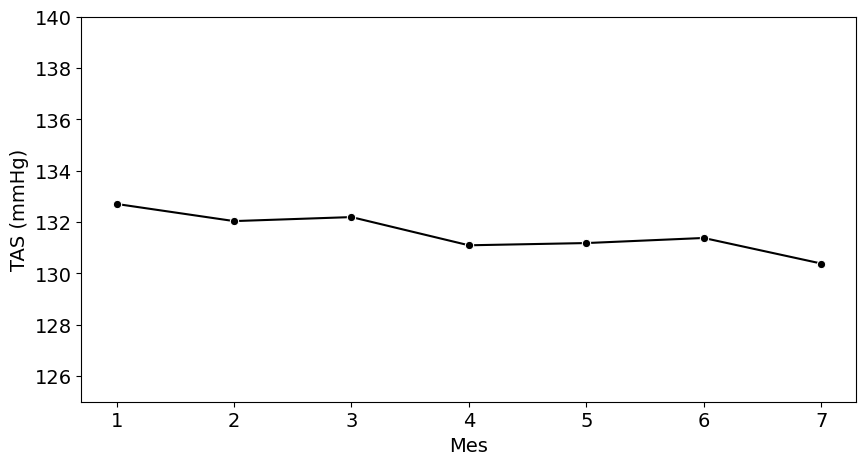
\includegraphics[scale=0.5]{img/TAS_vs_tpo.png}
	\caption{Evolución de la TAS promedio a lo largo del seguimiento}
	\label{TAS_vs_tpo}
\end{figure}

También resulta de interés observar la evolución de la TAS en el tiempo según la
edad basal y sexo de los pacientes. Como la variable edad es continua, para tal
fin, se la categorizó en 2 grupos ($< 59$ años y $>=$ 59 años, donde 59 es la
mediana de la edad de los pacientes estudiados). En la figura
(\ref{TAS_with_covs}) se observa que los perfiles promedios presentan (en
general) una pendiente decreciente, es decir, la TAS media disminuye con el
transcurso del seguimiento. Este comportamiento es similar para los grupos,
observando valores superiores de TAS para los pacientes de sexo masculino y para
los pacientes mayores de 59 años. 

\begin{figure}[H]
	\centering
	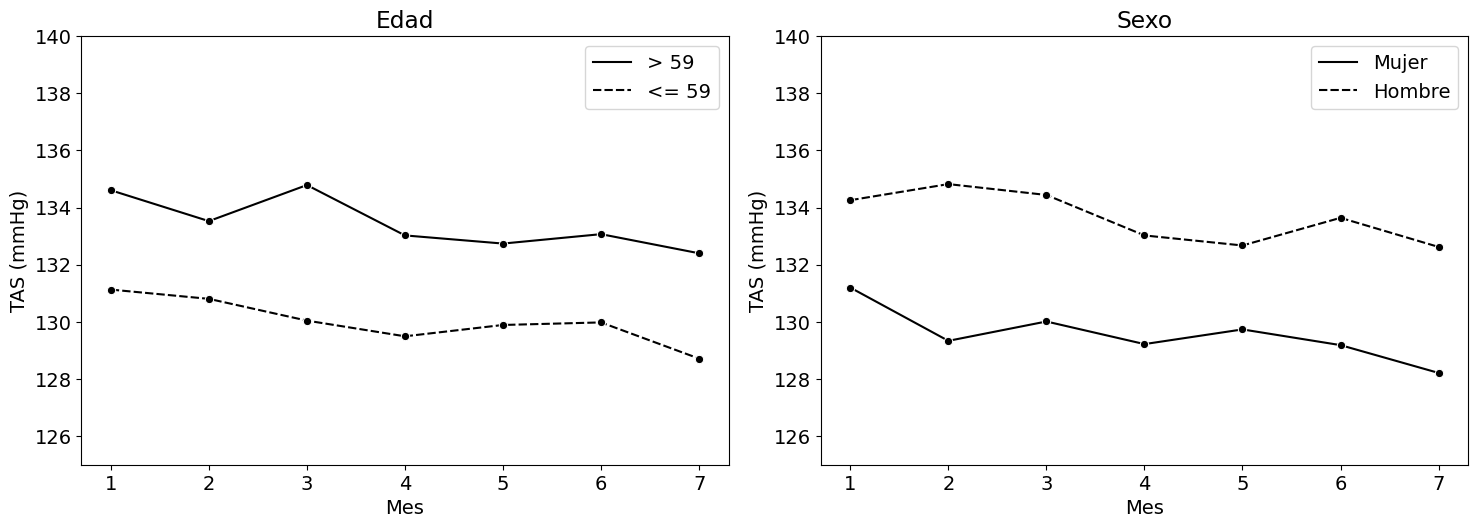
\includegraphics[scale=0.4]{img/TAS_vs_tpo_with_covs.png}
	\caption{Evolución de la TAS promedio a lo largo del seguimiento según sexo y edad}
	\label{TAS_with_covs}
\end{figure}

Para visualizar la relación entre la adherencia al tratamiento, el tiempo de
seguimiento y la TAS media, los gráficos de perfiles promedio no resultan
adecuados. La covariable ``adherencia al tratamiento'' es una CVT y, en
consecuencia, para cada individuo, puede presentar distintos valores en cada
ocasión, es decir, los pacientes no mantienen un perfil constante a lo largo del
tiempo. En una primera instancia, es posible realizar un diagrama de dispersión
entre la TAS y el tiempo (mes) según adherencia. Para poder observar con mayor
claridad la relación entre estas variables se utiliza la técnina ``jitter'', la
cual agrega un pequeño desplazamiento en los puntos, evitando que queden
perfectamente solapados. A partir de la figura (\ref{TAS_with_adh_scatter}), se
puede notar que esta manera de visualizar el efecto de la adherencia sobre la
TAS resulta confusa.

\begin{figure}[H]
	\centering
	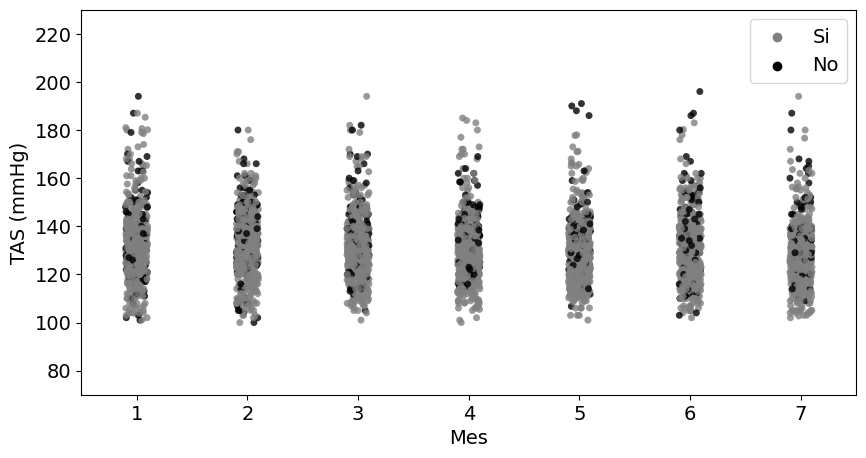
\includegraphics[scale=0.5]{img/TAS_vs_tpo_with_adherencia_scatter.png}
	\caption{Valores de la TAS a través del tiempo según adherencia}
	\label{TAS_with_adh_scatter}
\end{figure}

Como una alternativa a la presentada previamente, se propone realizar un gráfico
de perfiles promedio convirtiendo a la CVT (adherencia) en una CVNT, para que de
esta manera, cada paciente pertenezca únicamente a un sólo grupo durante todo el
período del estudio. Para esto, se dividieron a los pacientes según la cantidad
de meses que adhirieron al tratamiento, formando los grupos: 3 meses o menos
(adherencia baja), entre 4 y 6 meses (adherencia media/alta) o todos los meses
(adherencia perfecta). En la figura (\ref{TAS_with_adh}) se puede observar que
para el grupo de pacientes que adhirieron al tratamiento 3 meses o menos, la TAS
presenta una leve pendiente creciente a lo largo del estudio. Para los otros 2
grupos, la TAS disminuye a lo largo del seguimiento, observándose una
disminución mayor para el grupo de pacientes que adhirieron la totalidad de los
meses.

\begin{figure}[H]
	\centering
	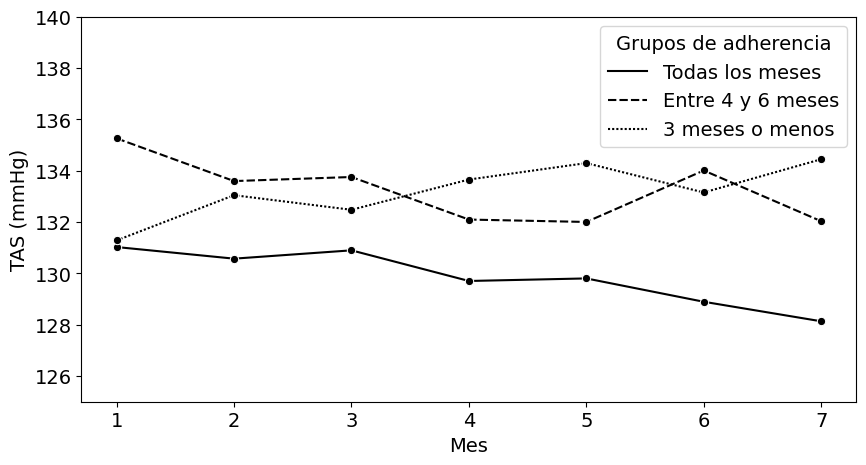
\includegraphics[scale=0.5]{img/TAS_vs_tpo_with_adherencia.png}
	\caption{TAS a través del tiempo según perfiles de adherencia al tratamiento}
	\label{TAS_with_adh}
\end{figure}

\subsection{Evaluación de la exogeneidad}
\label{evaluacion de la exogeneidad}

Para evaluar la exogeneidad de la variable adherencia al tratamiento es
necesario verificar el supuesto de independencia condicional descripto en
(\ref{seccion_de_exogeneidad}). Esto puede realizarse ajustando un modelo para
cada ocasión, en el que se considere a la variable adherencia como variable
respuesta, y como variables explicativas a la TAS y la adherencia en ocasiones
previas. Si, en estos modelos, las variables referentes a la TAS registrada en
ocasiones previas no resultan ser significativas, puede decirse que la
adherencia es una CVT exógena. Cómo la CVT adherencia es una variable
dicotómica, se ajustan modelos de regresión logística.

Para ajustar estos modelos se utilizarán como variables explicativas a la
adherencia y la TAS en el mes anterior, ya que se asume que las mediciones más
cercanas entre sí están más correlacionadas y tambien se utilizarán la
adherencia y la TAS promedio desde el inicio hasta 2 meses antes, de esta manera
se puede utilizar toda la información del estudio. El modelo para la ocasión $j$
($j = 2, ..., 7$) resulta:

$ 
	logit(P(adherencia_j=1)) = \beta_0 + \beta_1\ adherencia_{j-1} + \beta_2\ TAS_{j-1}
	+ \beta_3\ \overline{adherencia}_{j-2} + \beta_4\ \overline{TAS}_{j-2}
$

En la tabla (\ref{exog_table}) se presentan los valores de los coeficientes
estimados en cada modelo y entre paréntesis la probabilidad asociada a cada
coefiente (referente al test parcial $\left. H_0\right) Bk=0, k = 1, 2, 3, 4$).
Como se puede notar, en ninguna ocasión la adherencia depende de valores
anteriores de la TAS (cuando se controla por los valores previos de la
adherencia), por lo tanto puede considerarse como una covariable exógena.

\begin{table}[H]
	\centering
	\caption{Estimación de coeficientes de los modelos logit y sus respectivas probabilidades asociadas}
	\label{exog_table}
	\begin{tabular}{*{5}{|c}|}
		\hline
		mes\ (j) & $adherencia_{ij-1}$ & $\overline{adherencia}_{ij-2}$ & $TAS_{ij-1}$ &
		$\overline{TAS}_{ij-2}$ \\
		\hline
		\hline
		$2$ & $1.9302\ (<0.001)$ & $-$ & $0.0057\ (0.45)$ & $-$ \\
		$3$ & $2.3047\ (<0.001)$ & $0.5683\ (0.044)$ & $-0.0088\ (0.343)$ &
		$0.0075\ (0.419)$ \\
		$4$ & $1.9689\ (<0.001)$ & $1.0734\ (0.002)$ & $0.0138\ (0.17)$ &
		$-0.017\ (0.138)$ \\
		$5$ & $2.2945\ (<0.001)$ & $1.0617\ (0.007)$ & $0.0092\ (0.441)$ &
		$-0.0141\ (0.307)$ \\
		$6$ & $2.2741\ (<0.001)$ & $1.0698\ (0.015)$ & $-0.0008\ (0.938)$ &
		$<0.0001\ (0.996)$ \\
		$7$ & $2.5812\ (<0.001)$ & $1.4609\ (0.003)$ & $-0.0005\ (0.966)$ &
		$-0.0072\ (0.678)$ \\
		\hline
	\end{tabular}
\end{table}

\subsection{Modelos propuestos}

Se decidió plantear un modelo lineal de efectos mixtos (MLM) con ordenada
aleatoria y estructura de covariancia autorregresiva de orden 1. De esta manera,
se incorpora al modelo la correlación serial y el efecto entre pacientes
presente en los datos (ver anexo). Además, se incorpora el tiempo (mes) y como
covariables: el sexo, la edad y la adherencia al tratamiento. Esta última
variable, como se determinó en el punto anterior, es una CVT exógena y puede
incorporase al modelo de diferentes maneras. A continuación se presentan 6
modelos que surgen de plantear las distintas formas de incorporar la CVT
adherencia al tratamiento al MLM.

\subsubsection{Incorporación de la CVT como CNVT}

Hay diversas formas de convertir una CVT en CNVT. En este apartado se
presentarán dos que resultan de interés para el estudio:

\begin{itemize}
	\item adherencia perfecta (si/no).
	\item proporción de adherencia durante todo el seguimiento.
\end{itemize}

\paragraph{Adherencia perfecta} \mbox{}

Una de las transformaciones que puede aplicarse sobre la covariable adherencia
al tratamiento es convertirla en una variable dicotómica fija, cuyo valor es 1
si el paciente adhirió en todo el seguimiento y 0 en otro caso. El modelo
resulta:

\begin{equation}
	\label{modelo_1}
	Y_{ij} = \beta_0 + b_{0i} + \beta_1\ sexo_i + \beta_2\ edad_i + \beta_3\ adherencia\ perfecta_i
	+ \beta_4\ mes_j + \varepsilon_{ij}
\end{equation}

Se supone que $\bm{\varepsilon}_i$ y $b_{0i}$ son independientes.

\[ 
	\bm{\varepsilon}_i = \begin{pmatrix} \varepsilon_{i1} \\ \vdots \\ \varepsilon_{in} \end{pmatrix} \sim N_{n}(0, \bm{R}_i)
	\quad
	b_{0i} \sim N(0, Var(b_{0i}))
\]

Donde $\bm{R}_i$, matriz de variancias y covariancias del vector
$\bm{\varepsilon}_{i}$, se supone AR(1).

\begin{table}[H]
	\centering
	\caption{Parámetros estimados y medidas de bondad de ajuste del Modelo 1 que incorpora la CVT como Adherencia perfecta (CNVT)}
	\label{modelo_1_tabla}
	
    \begin{tabular}{*{5}{|c}|}
        \hline
        \multicolumn{3}{|c}{Log-Likelihood} & \multicolumn{2}{|c|}{-15377.6} \\
        \multicolumn{3}{|c}{AIC} & \multicolumn{2}{|c|}{30773.19} \\
        \multicolumn{3}{|c}{BIC} & \multicolumn{2}{|c|}{30829.66} \\
        \hline
        Covariable				   & Coef.                         & Std. Err.                  & z                           & $P<|z|$  \\
        \hline
	    $intercepto$ & 122,247 & 2,494 & 49,007 & $<0.001$ \\
	    $sexo_i$ & 3,742 & 0,751 & 4,986 & $<0.001$ \\
	    $edad_i$ & 0,166 & 0,039 & 4,292 & $<0.001$ \\
	    $adherencia_{ij}$ & -1,322 & 1,121 & -1,179 & $0.238$ \\
	    $mes_j$ & 0,394 & 0,236 & 1,671 & $0.095$ \\
	    $mes_j\ adherencia_{ij}$ & -0,832 & 0,26 & -3,2 & $0.001$ \\
        \hline
    \end{tabular}

\end{table}

En base a los resultados presentados en la tabla (\ref{modelo_1_tabla}),
controlando por el resto de las variables, los pacientes que adhieren siempre a
lo largo del seguimiento presentan una TAS promedio menor que los pacientes que
adhieren a veces o no adhieren en ningún momento. Esta diferencia es constante
en el tiempo.

\paragraph{Proporción de adherencia} \mbox{}

Otra manera de transformar a la CVT, conservando más información, es calcular la
proporción de adherencia al final del seguimiento. Por ejemplo, si un paciente
manifestó adherir al tratamiento en 5 de las 7 visitas, entonces la proporción
de adherencia es: $5/7= 0.71$. El modelo resulta:

\begin{equation}
	\label{modelo_2}
	Y_{ij} = \beta_0 + b_{0i} + \beta_1\ sexo_i + \beta_2\ edad_i + \beta_3\ \overline{adherencia}_i
	+ \beta_4\ mes_j + \varepsilon_{ij}
\end{equation}

Se supone que $\bm{\varepsilon}_i$ y $b_{0i}$ son independientes.

\[ 
	\bm{\varepsilon}_i = \begin{pmatrix} \varepsilon_{i1} \\ \vdots \\ \varepsilon_{in} \end{pmatrix} \sim N_{n}(0, \bm{R}_i)
	\quad
	b_{0i} \sim N(0, Var(b_{0i}))
\]

Donde $\bm{R}_i$, matriz de variancias y covariancias del vector
$\bm{\varepsilon}_{i}$, se supone con AR(1).

\begin{table}[H]
	\centering
	\caption{Parámetros estimados y medidas de bondad de ajuste del Modelo 2 que incorpora la CVT como Proporción de adherencia (CNVT)}
	\label{modelo_2_tabla}
	
    \begin{tabular}{*{5}{|c}|}
        \hline
        \multicolumn{3}{|c}{Log-Likelihood} & \multicolumn{2}{|c|}{-15415.08} \\
        \multicolumn{3}{|c}{AIC} & \multicolumn{2}{|c|}{30850.16} \\
        \multicolumn{3}{|c}{BIC} & \multicolumn{2}{|c|}{30912.9} \\
        \hline
        Covariable				   & Coef.                         & Std. Err.                  & z                           & $P<|z|$  \\
        \hline
	    $intercepto$ & 121,926 & 2,376 & 51,309 & $<0.001$ \\
	    $sexo_i$ & 3,801 & 0,741 & 5,129 & $<0.001$ \\
	    $edad_i$ & 0,176 & 0,038 & 4,589 & $<0.001$ \\
	    $adherencia\ perfecta_i$ & -2,491 & 1,177 & -2,117 & $0.035$ \\
	    $mes_j$ & -0,197 & 0,149 & -1,321 & $0.186$ \\
	    $mes_j\ adherencia\ perfecta_i$ & -0,272 & 0,212 & -1,279 & $0.201$ \\
        \hline
    \end{tabular}

\end{table}

En base a los resultados presentados en la tabla (\ref{modelo_2_tabla}),
controlando por el resto de las variables, a mayor proporción de adherencia
durante el seguimiento menores valores de TAS promedio.

\subsubsection{Incorporación de la CVT sin modificación}

Como se observó en el punto (\ref{evaluacion de la exogeneidad}), la CVT
adherencia al tratamiento es exógena y, en consecuencia, puede incorporarse en
su forma original al modelo. El MLM resulta en:

\begin{equation}
	\label{modelo_3}
	Y_{ij} = \beta_0 + b_{0i} + \beta_1\ sexo_i + \beta_2\ edad_i + \beta_3\ adherencia_{ij}
	+ \beta_4\ mes_j + \varepsilon_{ij}
\end{equation}

Se supone que $\bm{\varepsilon}_i$ y $b_{0i}$ son independientes.

\[ 
	\bm{\varepsilon}_i = \begin{pmatrix} \varepsilon_{i1} \\ \vdots \\ \varepsilon_{in} \end{pmatrix} \sim N_{n}(0, \bm{R}_i)
	\quad
	b_{0i} \sim N(0, Var(b_{0i}))
\]

Donde $\bm{R}_i$, matriz de variancias y covariancias del vector
$\bm{\varepsilon}_{i}$, se supone con AR(1).

\begin{table}[H]
	\centering
	\caption{Parámetros estimados y medidas de bondad de ajuste del Modelo 3 que incorpora la Adherencia al tratamiento sin transformar}
	\label{modelo_3_tabla}
	
    \begin{tabular}{*{5}{|c}|}
        \hline
        \multicolumn{3}{|c}{Log-Likelihood} & \multicolumn{2}{|c|}{-15403.63} \\
        \multicolumn{3}{|c}{AIC} & \multicolumn{2}{|c|}{30825.27} \\
        \multicolumn{3}{|c}{BIC} & \multicolumn{2}{|c|}{30881.73} \\
        \hline
        Covariable				   & Coef.                         & Std. Err.                  & z                           & $P<|z|$  \\
        \hline
	    $intercepto$ & 122,405 & 2,954 & 41,441 & $<0.001$ \\
	    $sexo_i$ & 3,718 & 0,751 & 4,949 & $<0.001$ \\
	    $edad_i$ & 0,17 & 0,039 & 4,391 & $<0.001$ \\
	    $\overline{adherencia}_i$ & -1,598 & 2,33 & -0,686 & $0.493$ \\
	    $mes_j$ & 0,523 & 0,365 & 1,431 & $0.152$ \\
	    $mes_j\ \overline{adherencia}_i$ & -1,052 & 0,427 & -2,463 & $0.014$ \\
        \hline
    \end{tabular}

\end{table}

En base a los resultados presentados en la tabla (\ref{modelo_3_tabla}),
controlando por el resto de las variables y para un momento de tiempo
determinado, los pacientes que adhieren al tratamiento presentan una TAS
promedio menor que los pacientes que no adhieren al tratamiento.

\subsubsection{Incorporación de la CVT considerando la covariable rezagada}

Puede pensarse que el efecto de la adherencia al tratamiento no es inmediato y
entonces se desea considerar la adherencia al tratamiento observada en el mes
anterior a la visita (rezago $k=1$). A continuación, se presenta el MLM
resultante:

\begin{equation}
	\label{modelo_4}
	Y_{ij} = \beta_0 + b_{0i} + \beta_1\ sexo_i + \beta_2\ edad_i + \beta_3\ adherencia_{ij-1}
	+ \beta_4\ mes_j + \varepsilon_{ij}
\end{equation}

Se supone que $\bm{\varepsilon}_i$ y $b_{0i}$ son independientes.

\[ 
	\bm{\varepsilon}_i = \begin{pmatrix} \varepsilon_{i1} \\ \vdots \\ \varepsilon_{in} \end{pmatrix} \sim N_{n}(0, \bm{R}_i)
	\quad
	b_{0i} \sim N(0, Var(b_{0i}))
\]

Donde $\bm{R}_i$, matriz de variancias y covariancias del vector
$\bm{\varepsilon}_{i}$, se supone con AR(1).

\begin{table}[H]
	\centering
	\caption{Parámetros estimados y medidas de bondad de ajuste del Modelo 4 que incorpora la Adherencia al tratamiento en la visita anterior}
	\label{modelo_4_tabla}
	
    \begin{tabular}{*{5}{|c}|}
        \hline
        \multicolumn{3}{|c}{Log-Likelihood} & \multicolumn{2}{|c|}{-15422.5} \\
        \multicolumn{3}{|c}{AIC} & \multicolumn{2}{|c|}{30865.0} \\
        \multicolumn{3}{|c}{BIC} & \multicolumn{2}{|c|}{30927.74} \\
        \hline
        Covariable				   & Coef.                         & Std. Err.                  & z                           & $P<|z|$  \\
        \hline
	    $intercepto$ & 121,125 & 2,388 & 50,713 & $<0.001$ \\
	    $sexo_i$ & 3,869 & 0,752 & 5,147 & $<0.001$ \\
	    $edad_i$ & 0,162 & 0,039 & 4,196 & $<0.001$ \\
	    $adherencia_{ij-1}$ & 0,189 & 0,815 & 0,232 & $0.817$ \\
	    $mes_j$ & 0,064 & 0,179 & 0,359 & $0.719$ \\
	    $mes_j\ adherencia_{ij-1}$ & -0,443 & 0,215 & -2,065 & $0.039$ \\
        \hline
    \end{tabular}

\end{table}

En base a los resultados presentados en la tabla (\ref{modelo_4_tabla}),
controlando por el resto de las variables y para un momento de tiempo
determinado, no se observan diferencias significativas en la TAS promedio entre
los pacientes que adhieren al tratamiento en la visita anterior y los que no
adhirieron.

\subsubsection{Incorporación de la CVT como función de covariables rezagadas}

Puede pensarse que el efecto de la adherencia al tratamiento en la TAS no sólo
depende del mes anterior sino también del comportamiento del paciente en las
visitas previas. Por lo tanto, se decidió calcular para cada paciente la
proporción de adherencia al tratamiento hasta el mes actual. Por ejemplo, si
hasta la visita del mes 5 el paciente manifestó adherir al tratamiento en 3 de
ellas y en 2 no, la proporción de adherencia al tratamiento al mes 5 es de 3/5.
Esta nueva covariable resulta también ser una CVT.

A continuación, se presenta el MLM resultante:

\begin{equation}
	\label{modelo_5}
	Y_{ij} = \beta_0 + b_{0i} + \beta_1\ sexo_i + \beta_2\ edad_i + \beta_3\ \overline{adherencia}_{ij}
	+ \beta_4\ mes_j + \varepsilon_{ij}
\end{equation}

Se supone que $\bm{\varepsilon}_i$ y $b_{0i}$ son independientes.

\[ 
	\bm{\varepsilon}_i = \begin{pmatrix} \varepsilon_{i1} \\ \vdots \\ \varepsilon_{in} \end{pmatrix} \sim N_{n}(0, \bm{R}_i)
	\quad
	b_{0i} \sim N(0, Var(b_{0i}))
\]

Donde $\bm{R}_i$, matriz de variancias y covariancias del vector
$\bm{\varepsilon}_{i}$, se supone con AR(1).

\begin{table}[H]
	\centering
	\caption{Parámetros estimados y medidas de bondad de ajuste del Modelo 5 que incorpora la Proporción de adherencia al tratamiento hasta la visita actual}
	\label{modelo_5_tabla}
	
    \begin{tabular}{*{5}{|c}|}
        \hline
        \multicolumn{3}{|c}{Log-Likelihood} & \multicolumn{2}{|c|}{-15409.38} \\
        \multicolumn{3}{|c}{AIC} & \multicolumn{2}{|c|}{30838.77} \\
        \multicolumn{3}{|c}{BIC} & \multicolumn{2}{|c|}{30901.51} \\
        \hline
        Covariable				   & Coef.                         & Std. Err.                  & z                           & $P<|z|$  \\
        \hline
	    $intercepto$ & 123,107 & 2,586 & 47,603 & $<0.001$ \\
	    $sexo_i$ & 3,721 & 0,749 & 4,966 & $<0.001$ \\
	    $edad_i$ & 0,177 & 0,039 & 4,574 & $<0.001$ \\
	    $\overline{adherencia}_{ij}$ & -3,247 & 1,421 & -2,285 & $0.022$ \\
	    $mes_j$ & 0,382 & 0,306 & 1,248 & $0.212$ \\
	    $mes_j\ \overline{adherencia}_{ij}$ & -0,835 & 0,355 & -2,348 & $0.019$ \\
        \hline
    \end{tabular}

\end{table}

En base a los resultados presentados en la tabla (\ref{modelo_5_tabla}),
controlando por el resto de las variables y para un momento de tiempo
determinado, a mayor proporción de adherencia al tratamiento hasta ese momento,
se esperan menores valores de TAS promedio.

\subsubsection{Incorporación de la CVT, dividiendo su efecto en dos componentes}

Como se presentó en el apartado (\ref{Dividiendo efecto entre-unidad y efecto
intra-unidad}), el efecto de la CVT puede descomponerse en dos componentes:
efecto intra paciente y efecto entre pacientes. Puesto que la variable
adherencia es dicotómica, se considera el efecto intra paciente solamente con
$X_{ij}$. El MLM resultante es:

\begin{equation}
	\label{modelo_6}
	Y_{ij} = \beta_0 + b_{0i} + \beta_1\ sexo_i + \beta_2\ edad_i + \beta_3\ adherencia_{ij}
	+ \beta_4\ \overline{adherencia}_i + \beta_5\ mes_j + \varepsilon_{ij}
\end{equation}

Se supone que $\bm{\varepsilon}_i$ y $b_{0i}$ son independientes.

\[ 
	\bm{\varepsilon}_i = \begin{pmatrix} \varepsilon_{i1} \\ \vdots \\ \varepsilon_{in} \end{pmatrix} \sim N_{n}(0, \bm{R}_i)
	\quad
	b_{0i} \sim N(0, Var(b_{0i}))
\]

Donde $\bm{R}_i$, matriz de variancias y covariancias del vector
$\bm{\varepsilon}_{i}$, se supone con AR(1).

\begin{table}[H]
	\centering
	\caption{Parámetros estimados y medidas de bondad de ajuste del Modelo 6 que incorpora dos componentes para la adherencia al tratamiento}
	\label{modelo_6_tabla}
	
    \begin{tabular}{*{5}{|c}|}
        \hline
        \multicolumn{3}{|c}{Log-Likelihood} & \multicolumn{2}{|c|}{-15382.25} \\
        \multicolumn{3}{|c}{AIC} & \multicolumn{2}{|c|}{30782.5} \\
        \multicolumn{3}{|c}{BIC} & \multicolumn{2}{|c|}{30838.96} \\
        \hline
        Covariable				   & Coef.                         & Std. Err.                  & z                           & $P<|z|$  \\
        \hline
	    $intercepto$ & 125,696 & 2,599 & 48,36 & $<0.001$ \\
	    $sexo_i$ & 3,713 & 0,751 & 4,943 & $<0.001$ \\
	    $edad_i$ & 0,17 & 0,039 & 4,388 & $<0.001$ \\
	    $adherencia_{ij}$ & -4,22 & 0,602 & -7,008 & $<0.001$ \\
	    $\overline{adherencia}_i$ & -1,622 & 1,692 & -0,958 & $0.338$ \\
	    $mes_j$ & -0,291 & 0,101 & -2,873 & $0.004$ \\
        \hline
    \end{tabular}

\end{table}

En base a los resultados presentados en la tabla (\ref{modelo_6_tabla}),
controlando por el resto de las variables y para un momento de tiempo
determinado, la proporción de aherencia en todo el seguimiento no resulta ser
signficatva. En cambio, la adherencia en cada visita si lo es, evidenciando que
la TAS promedio es menor para los pacientes que adhieren al tratamiento en la
visita que para los que no.

\subsubsection{Comparación de los modelos propuestos}

A continuación, en la tabla \ref{comparacion}, se presentan para cada uno de los
6 modelos ajustados la forma en la que se incorporó la covariable adherencia al
tratamiento, el valor estimado del coeficiente que acompaña a la covariable
conjuntamente con la probabilidad asociada y los valores de los criterios de
información de Akaike (AIC) y Bayesiano de Schwarz (BIC).

\begin{table}[H]
	\centering
	\caption{Resumen de los modelos ajustados}
	\label{comparacion}
	\begin{tabular}{|c|p{5cm}|p{5cm}|c|c|}
		\hline
		Modelo & Forma de incorporar la adherencia al tratamiento & Parámetro estimado asociado a la adherencia(prob asoc) & AIC & BIC \\
		\hline
		Modelo 1 & Adherencia perfecta (CNVT) & $-3.608\ (<0.001)$ & $30819.66$ & $30869.85$ \\
		\hline
		Modelo 2 & Proporción de adherencia (CNVT) & $-5.806\ (<0.001)$ & $30829.33$ & $30879.52$ \\
		\hline
		Modelo 3 & Adherencia al tratamiento sin transformar & $-4.423\ (<0.001) $ & $30781.42$ & $30831.61$ \\
		\hline
		Modelo 4 & Adherencia al tratamiento en la visita anterior & $-0.854\ (0.076)$ & $30839.53$ & $30889.72$ \\
		\hline
		Modelo 5 & Proporción de adherencia al tratamiento hasta la visita actual & $-5.12\ (<0.001)$ & $30815.82$ & $30866.01$ \\
		\hline
		\multirow{2}{*}{Modelo 6}
		& Adherencia al tratamiento sin transformar & $-4.22\ (<0.001)$ & \multirow{2}{*}{30782.5} & \multirow{2}{*}{30838.96} \\
		\cline{2-3}
		& Proporción de adherencia (CNVT) & $-0,291\ (0.338)$ & & \\
		\hline
	\end{tabular}
\end{table}

En la tabla (\ref{comparacion}) se puede observar que, basándose en el AIC y el
BIC, el modelo que mejor ajusta a los datos es el modelo 3 (\ref{modelo_3}),
este modelo incorpora la CVT en su forma natural sin aplicarse ninguna
transformación. El segundo modelo que mejor ajusta los datos es el modelo 6
(\ref{modelo_6}), el cual también incorpora la covariable en su forma natural y
además incorpora una transformación CNVT de ésta para dividir su efecto y
facilitar la interpretación de sus parámetros.

\newpage

\section{Consideraciones finales}

Los datos que surgen de estudios longitudinales pueden ser analizados mediante
modelos lineales mixtos. En este tipo de estudios es frecuente contar con
variables independientes que pueden ser fijas a lo largo de todo el período o
bien puedan variar a lo largo del seguimiento. Estas covariables que varían con
el tiempo son variables independientes que incluyen tanto la variación
intra-sujeto y la variación entre-sujetos.

La relación entre la covariable que varía en el tiempo y la variable respuesta
puede estar confundida por valores anteriores y/o posteriores de la covariable
y, en consecuencia, esto puede conducir a inferencias engañosas sobre los
parámetros del modelo.

En esta tesina se presentaron diferentes definiciones y tipos de covariables que
varían en el tiempo, específicamente se introdujo el concepto de covariable
endógena y exógena. También se describió una forma empírica de evaluar esta
clasificación.

Se presentaron diferentes formas de introducir una covariable que varía en el
tiempo exógena al modelo lineal mixto, ya sea en su formato original o bien
mediante transformaciones. Estos conceptos fueron aplicados a un conjunto de
datos que surge del programa de atención y control de pacientes hipertensos de
Fundación ECLA.

Uno de los objetivos que persiguió este estudio observacional fue evaluar si la
adherencia al tratamiento (covariable que varía en el tiempo) influía en los
valores de la TAS a lo largo del seguimiento. En primer lugar se evaluó la
exogeneidad de ésta covariable, luego se presentaron diferentes formas de
introducirla al modelo lineal mixto dando lugar a 6 propuestas diferentes.
Posteriormente, se compararon estas propuestas y se arribó a un modelo final en
el que se incorpora a la covariable adherencia en su formato original sin
realizar transformaciones. En este modelo se concluye que, controlando por el
resto de las variables y para un momento de tiempo determinado, los pacientes
que adhieren al tratamiento presentan una TAS promedio menor que los pacientes
que no adhieren al tratamiento.

Se propone como sugerencia para futuros estudios evaluar la incorporación de
covariables continuas que varían en el tiempo, ya que en este trabajo la
covariable de interés es dicotómica. También se propone evaluar el tratamiento
de covariables que varian en el tiempo que resultan ser endógenas al evaluar su
condición.

\newpage

\section{Anexo}

\begin{figure}[H]
	\centering
	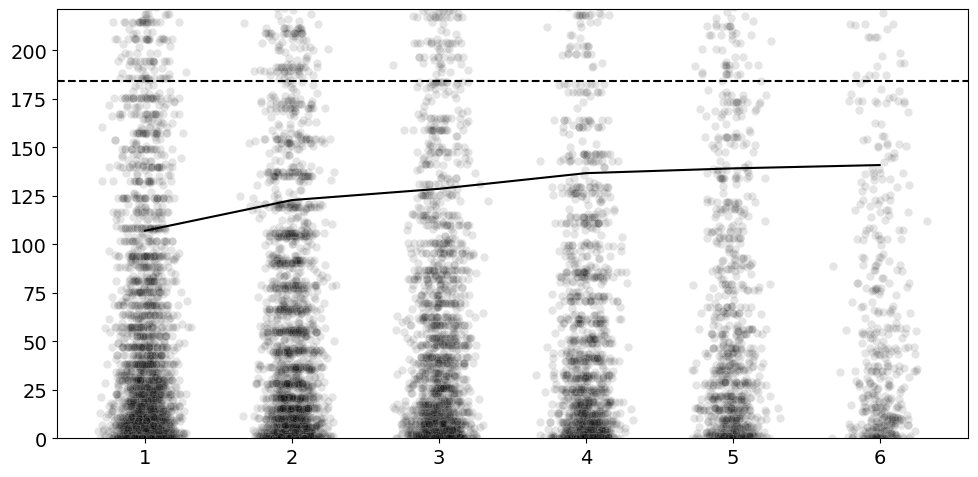
\includegraphics[scale=0.4]{img/semivariogram.png}
	\caption{Semivariograma muestral}
	\label{semivariogram}
\end{figure}

\begin{figure}[H]
	\centering
	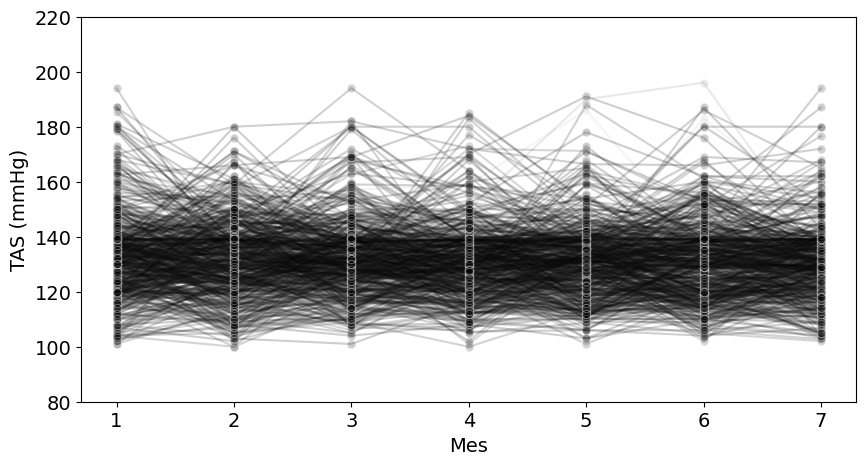
\includegraphics[scale=0.5]{img/TAS_vs_tpo_perfiles_individuales.png}
	\caption{Evolución de la TAS a lo largo del tiempo para cada paciente}
	\label{perfiles_individuales}
\end{figure}


\newpage
\nocite{*}
\renewcommand{\refname}{Bibliografía}
\bibliography{Bibliografia}

\end{document}